\part{Amendment 8: Where the Leaked Signal Lives}

\chapter{Why a follow-up, and what was known}
\label{r:ch:a8-why}

Study~2 established \emph{that} crop-level splitting inflates accuracy and that the inflation is leakage, but neither
registered mechanism test isolated \emph{how} models use it. Two observations pointed the way. Leak models kept most of
their advantage on backgrounds transplanted from unseen fields, which suggested a carrier inside the cell region rather
than in the background. And the ConvNeXt-T adversary had been evaded, so the gradient-reversal arm had only one usable
architecture.

Amendment~8 (\artifact{PREREGISTRATION_STUDY2_AMENDMENT8.md}, commit \texttt{\FollowupCommit}, \FollowupTime) registered
eight new hypotheses after the Study~2 analysis and before any follow-up model was trained or any follow-up analysis was
run on existing outputs. It states what was known and what was not: every registered Study~2 output was known, including
transplant condition means and gradient-reversal sweep means; no per-cell CRIC result by slide composition, no ablated
image evaluation, no erased-feature evaluation, no Grad-CAM map, and no model trained with masked backgrounds, colour
augmentation, stain normalisation, or the linear adversary had been seen. F1--F8 form their own Holm family, separate from
H1--H5, whose verdicts the amendment does not touch.

\begin{figure}[H]
\centering
\begin{adjustbox}{max width=\textwidth}
\begin{tikzpicture}[node distance=4mm and 6mm]
\node[box=34mm] (cric) {\textbf{F1} CRIC slide context\\\footnotesize saved predictions, CPU only};
\node[box=34mm, right=of cric] (abl) {\textbf{F2} test-time ablations + Grad-CAM\\\footnotesize 160 saved 2C models};
\node[gold=34mm, right=of abl] (car) {\textbf{F3, F4} carrier factorial\\\footnotesize 480 new runs, fresh seeds};
\node[box=34mm, below=8mm of cric] (leace) {\textbf{F5} LEACE erasure\\\footnotesize 480 saved Phase 1 models};
\node[gold=34mm, right=of leace] (norm) {\textbf{F6} stain normalisation\\\footnotesize 160 new runs};
\node[gold=34mm, right=of norm] (lin) {\textbf{F7} linear adversary\\\footnotesize 300 new runs};
\node[done=110mm, below=8mm of norm] (pool) {\textbf{F8} pooled dose-response of the gap on recoverability over the in-regime levels of F5, F6, F7};
\draw[flow] (leace.south) -- (leace.south |- pool.north);
\draw[flow] (norm.south) -- (pool.north);
\draw[flow] (lin.south) -- (lin.south |- pool.north);
\node[note, above=1mm of abl] {where the leak lives};
\node[note, above=1mm of norm] {does the gap track the fingerprint?};
\end{tikzpicture}
\end{adjustbox}
\caption{The eight Amendment~8 hypotheses. Blue arms reuse saved Study~2 artifacts (no retraining); gold arms train new
models on seeds no earlier arm used; F8 pools the three dose-response arms.}
\label{r:fig:followup-arms}
\end{figure}


\chapter{The eight follow-up designs}
\label{r:ch:a8-designs}

\section{F1: slide context in CRIC}

CRIC slide images contain cells of several classes (83\% of slides have more than one), so a test cell's training
siblings can carry a different label. For every cell, the \emph{context class} is the majority class of the other cells
of its slide (cells whose slide has no other cell, or a tied majority, are excluded). A \emph{discordant} cell's class
differs from its context class. If crop-level models apply a slide-level label prior, discordant cells should receive more
probability on the context class when their slide was in training (P1) than when it was not (P2). F1 is that within-cell
difference over the 120 saved CRIC P1 and P2 runs, with a percentile cluster bootstrap over slides (10,000 replicates).

\begin{figure}[H]
\centering
\begin{adjustbox}{max width=\textwidth}
\begin{tikzpicture}[node distance=4mm and 6mm, cell/.style={circle,draw=CytoInk!60,minimum size=5mm,inner sep=0pt,font=\scriptsize}]
\node[draw=CytoBlue, rounded corners, minimum width=52mm, minimum height=26mm, label={[font=\small]above:One CRIC slide image}] (slide) {};
\node[cell, fill=SerBlue!35] at ($(slide.center)+(-18mm,6mm)$) {N};
\node[cell, fill=SerBlue!35] at ($(slide.center)+(-8mm,7mm)$) {N};
\node[cell, fill=SerBlue!35] at ($(slide.center)+(3mm,6mm)$) {N};
\node[cell, fill=SerBlue!35] at ($(slide.center)+(14mm,7mm)$) {N};
\node[cell, fill=SerBlue!35] at ($(slide.center)+(-14mm,-5mm)$) {N};
\node[cell, fill=SerBlue!35] at ($(slide.center)+(-3mm,-6mm)$) {N};
\node[cell, fill=SerOrange!45, very thick] (target) at ($(slide.center)+(10mm,-6mm)$) {L};
\node[box=46mm, right=10mm of slide] (def) {Context class of the orange cell = majority of the \emph{other} cells = N.\\
Its own class L $\neq$ N: a \textbf{discordant} cell.};
\node[box=46mm, below=4mm of def] (test) {F1: $p$(N) for this cell under P1 (slide in training) minus under P2 (slide unseen); predicted $>0$.};
\node[done=46mm, below=4mm of test] (res) {Observed: \FoneEst~pp, the opposite sign.};
\draw[flow] (target) -- (def); \draw[flow] (def) -- (test); \draw[flow] (test) -- (res);
\end{tikzpicture}
\end{adjustbox}
\caption{How F1 defines a discordant cell. A slide-level label prior would pull discordant cells toward their slide's
majority class when the slide was seen in training; the models did the opposite.}
\label{r:fig:cric-context-diagram}
\end{figure}


\section{F2: carrier ablations at test time}

Each of the 160 saved 2C models is re-evaluated on its seed's common test set under six conditions rendered at native
resolution: original; greyscale; Reinhard stain transfer of the crop's LAB mean and standard deviation to those of the 2B
unseen same-class donor~\citep{reinhard2001color}; low-pass (Gaussian $\sigma=2$~px at the 224-px input); illumination
flattening (subtracting a $\sigma=16$~px Gaussian); and background replaced by the ImageNet mean. F2 asks whether stain
transfer shrinks the leak-minus-clean advantage. Grad-CAM~\citep{selvaraju2017gradcam} attribution outside the cell mask is
measured on the convolutional models and reported descriptively, with a random-head sanity check~\citep{adebayo2018sanity}.

\section{F3 and F4: carrier removal in training}

The 2C factorial is rerun on ten seeds never used for any model (1103, 1151, 1201, 1249, 1301, 1361, 1409, 1451, 1499, 1553)
under three conditions: the standard recipe; every training and test crop's background masked to the ImageNet mean; and
strong HED optical-density colour augmentation~\citep{tellez2019quantifying,ruifrok2001color} ($\alpha\in[0.8,1.2]$,
$\beta\in[-0.2,0.2]$ per stain channel, then brightness and contrast in $[0.8,1.2]$) during training. F3 asks whether leakage
survives with no background; F4 whether colour augmentation shrinks it. The standard condition is an independent
replication of H3.

\section{F5: rank-limited LEACE erasure}

\begin{figure}[H]
\centering
\begin{adjustbox}{max width=\textwidth}
\begin{tikzpicture}[node distance=4mm and 5mm]
\node[box=24mm] (ckpt) {Saved Phase 1 checkpoint\\\footnotesize hash-verified};
\node[box=24mm, right=of ckpt] (feat) {Features of all 4,049 crops\\\footnotesize eval transform};
\node[box=26mm, right=of feat] (white) {Whiten with $W=\Sigma^{-1/2}$\\\footnotesize training crops only};
\node[box=28mm, right=of white] (scatter) {Within-class between-parent scatter $S$; top-$r$ eigvecs of $WSW$};
\node[box=28mm, below=of scatter] (erase) {$x' = x - (x-\mu)\,W U_r U_r^\top W^{-1}$};
\node[box=24mm, left=of erase] (refit) {Refit linear class head\\\footnotesize logistic, C = 1};
\node[box=24mm, left=of refit] (acc) {Test accuracy\\\footnotesize P1 and P2 models};
\node[box=24mm, left=of acc] (probe) {Recoverability $R$\\\footnotesize probe split, same eraser};
\draw[flow] (ckpt) -- (feat); \draw[flow] (feat) -- (white); \draw[flow] (white) -- (scatter); \draw[flow] (scatter) -- (erase);
\draw[flow] (erase) -- (refit); \draw[flow] (refit) -- (acc); \draw[flow] (acc) -- (probe);
\end{tikzpicture}
\end{adjustbox}
\caption{Rank-limited LEACE erasure (F5). At full rank the projection is LEACE for the within-class parent indicator:
no linear function of the erased features covaries with it on the fitting data. Ranks 0, 4, 16, 64, and 256 give the dose.}
\label{r:fig:leace}
\end{figure}


Every saved Phase~1 P1 and P2 model (480) is re-evaluated: features of all crops are extracted, the within-class parent
directions of the model's own training crops are erased at ranks 0, 4, 16, 64, and 256~\citep{belrose2023leace}, the class
head is refitted, and test accuracy and recoverability are measured. The regime and manipulation check follow H5. F5 asks
whether erasure at the strongest in-regime rank reduces the P1 $-$ P2 gap.

\section{F6: stain-normalisation dose}

Every crop is Reinhard-normalised toward one dataset-wide reference at strength 0.5 and 1.0, in training, test, and probe
crops alike. ResNet-50, ConvNeXt-T, DenseNet-121, and EfficientNet-B0 are trained on P1 and P2 for the ten Study~2 seeds no
mechanism arm used; strength 0 is the matching Phase~1 run. F6 is the reduction in gap per unit of strength.

\section{F7: probe-matched linear adversary}

The 2A design with a different adversary (Figure~\ref{r:fig:adversary}): per-feature standardisation and one linear layer,
its own optimiser at $10^{-3}$, re-initialised every five epochs. ResNet-50, ConvNeXt-T, and DenseNet-121; $\lambda\in\{0,
0.1, 0.3, 1, 3\}$; P1 and P2; the same ten seeds as F6. F7 is the slope of gap on recoverability, as for H5.

\section{F8: pooled dose-response}

All included architecture-by-level cells of F5, F6, and F7, after their regimes and manipulation checks:
$\text{gap}\sim\text{cell}+R_{\text{pair}}+(1\mid\text{manipulation:seed})$. F8 is the slope.

\section{Recoverability, measured the same way everywhere}

$R$ for F5--F8 is computed with one GPU implementation of the registered logistic probe (sklearn's objective, C = 1,
standardised features, L-BFGS). On the 280 Study~2 gradient-reversal runs it agreed with the registered sklearn probe at
$r=\ProbeAgreement$ (Figure~\ref{r:fig:probe-agreement}).

\begin{figure}[H]
\centering
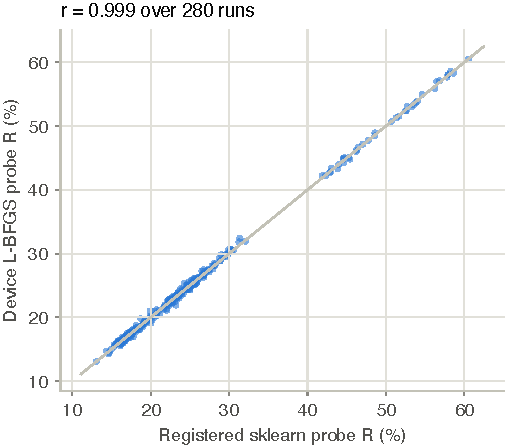
\includegraphics[width=0.55\textwidth]{probe_agreement.pdf}
\caption{Within-class recoverability from the registered sklearn probe and the device probe used for F5--F8, on the 280
Study~2 adversarial runs.}
\label{r:fig:probe-agreement}
\end{figure}

\chapter{Execution and the Amendment 9 fix}
\label{r:ch:a8-exec}

The new code was unit-tested on the workstation and, for GPU paths, on the host (13 tests, including a check that
full-rank erasure leaves no covariance between features and within-class parent identity, and that the device probe
matches sklearn to $10^{-3}$). A synthetic dry run of the registered models recovered every planted effect. Eleven smoke
tasks ran only on leak cells and single P1 runs; they confirmed that re-evaluated checkpoints reproduce their recorded
accuracy and that the linear adversary learns. The caches for masking, normalisation, and the ablations were built and
hashed, and the registration commit recorded every hash. The matrix of \RecFollowTasks\ tasks then ran from
\RecFollowStart\ to \RecFollowEnd\ without a failure.

\begin{warningbox}{Amendment 9: the preparer bug}
When the registered models were first run on the completed carrier arm, the R script stopped at F4: the preparer had
labelled all 160 standard-recipe runs as colour-augmented, because a missing colour augmentation (\texttt{None} in the run
record) became a NaN in a DataFrame row, and NaN is truthy. The script halted before writing any output, so no F3 or F4
estimate was seen. The condition is now read from each run record, a unit test covers it, and the fix was registered as
Amendment~9 (20 October, 01:25) before the corrected table was analysed. The synthetic dry run had bypassed the preparer,
which is why the bug was not caught earlier.
\end{warningbox}

\chapter{Follow-up results}
\label{r:ch:a8-results}

\small\begin{longtable}{lp{0.33\textwidth}rrrl}
\caption{The eight registered follow-up tests (one Holm family). Estimates are oriented so that the predicted direction is
positive.}\label{r:tab:a8-verdicts}\\
\toprule
& Question & Estimate & 95\% CI & Holm $p$ & Verdict \\
\midrule
\endfirsthead
\bottomrule
\endfoot
F1 & CRIC pull toward the slide's majority class & \FoneEst & \FoneLo\ to \FoneHi & \FonePholm & \notsupported \\
F2 & Stain transfer shrinks the leak effect & \FtwoEst & \FtwoLo\ to \FtwoHi & \FtwoPholm & \supported \\
F3 & Leak effect with backgrounds masked & \FthreeEst & \FthreeLo\ to \FthreeHi & \FthreePholm & \supported \\
F4 & Colour augmentation shrinks the leak effect & \FfourEst & \FfourLo\ to \FfourHi & \FfourPholm & \notsupported \\
F5 & LEACE erasure shrinks the gap & \FfiveEst & \FfiveLo\ to \FfiveHi & \FfivePholm & \notsupported \\
F6 & Stain normalisation shrinks the gap & \FsixEst & \FsixLo\ to \FsixHi & \FsixPholm & \notsupported \\
F7 & Gap tracks $R$ (linear adversary) & \FsevenEst & \FsevenLo\ to \FsevenHi & \FsevenPholm & \notsupported \\
F8 & Gap tracks $R$ (pooled) & \FeightEst & \FeightLo\ to \FeightHi & \FeightPholm & \notsupported \\
\end{longtable}

\section{The leak needs no background (F3)}

Trained and tested with every background replaced by a constant, leak models beat clean models by \FthreeEst~pp
(\FthreeLo--\FthreeHi; Holm $p$ \FthreePholm), at least as much as under the standard recipe on the same fresh seeds
(\CarrierStandard~pp), which also replicates H3 (\HthreeRepEst~pp, \HthreeRepLo--\HthreeRepHi). Masking changed the leak
effect by \MaskReductionEst~pp relative to standard training (\MaskReductionLo\ to \MaskReductionHi). At test time, removing
the background from the original 2C models' inputs left \RecBgKeep\% of their advantage.

\begin{figure}[H]
\centering
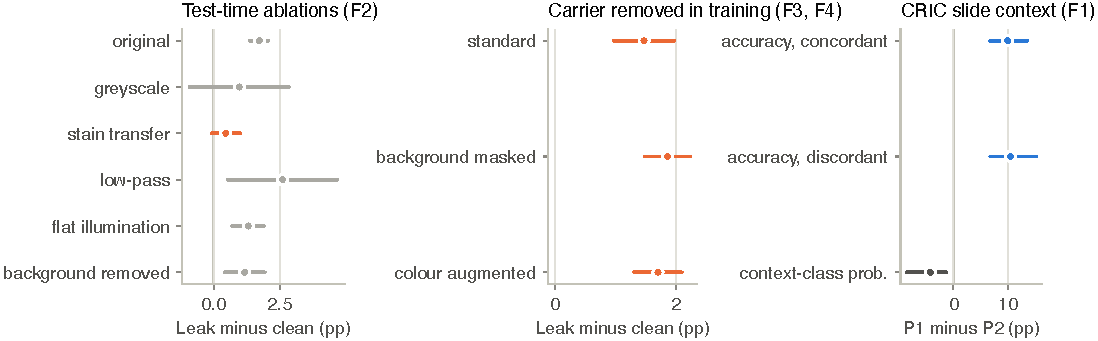
\includegraphics[width=\textwidth]{carriers.pdf}
\caption{Left: the leak advantage under each test-time ablation (F2 highlighted). Middle: the leak effect under each
training condition on fresh seeds (F3, F4). Right: CRIC within-cell accuracy gains by concordance, and the context-class
probability for discordant cells (F1).}
\label{r:fig:carriers}
\end{figure}

\begin{figure}[H]
\centering
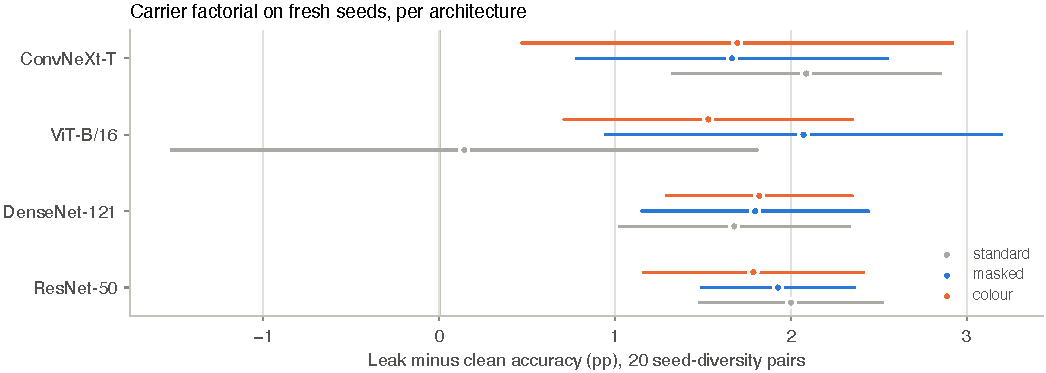
\includegraphics[width=\textwidth]{carrier_arch.pdf}
\caption{The carrier factorial per architecture.}
\label{r:fig:carrier-arch}
\end{figure}

{\scriptsize
\setlength{\tabcolsep}{3.5pt}
\begin{longtable}{llrrrrr}
\caption{Amendment 8 carrier factorial (fresh seeds, 10 per cell): accuracy per cell (percent) and the leak effect (pp).}\label{r:tab:carrier}\\
\toprule
Architecture & Condition & Leak high & Clean high & Leak low & Clean low & Leak effect \\
\midrule
\endfirsthead
\toprule
Architecture & Condition & Leak high & Clean high & Leak low & Clean low & Leak effect \\
\midrule
\endhead
\bottomrule
\endfoot
ResNet-50 & standard & 96.06\,$\pm$\,1.42 & 93.99\,$\pm$\,2.08 & 96.40\,$\pm$\,0.79 & 94.48\,$\pm$\,1.52 & 2.00 \\
 & masked & 95.46\,$\pm$\,1.19 & 93.42\,$\pm$\,1.26 & 95.69\,$\pm$\,1.36 & 93.87\,$\pm$\,1.37 & 1.92 \\
 & colour & 95.62\,$\pm$\,1.29 & 93.79\,$\pm$\,1.29 & 95.84\,$\pm$\,1.04 & 94.10\,$\pm$\,1.45 & 1.78 \\
DenseNet-121 & standard & 96.33\,$\pm$\,1.16 & 95.14\,$\pm$\,1.63 & 97.01\,$\pm$\,0.66 & 94.85\,$\pm$\,1.50 & 1.68 \\
 & masked & 95.59\,$\pm$\,1.32 & 94.21\,$\pm$\,1.00 & 96.19\,$\pm$\,0.87 & 93.99\,$\pm$\,1.84 & 1.79 \\
 & colour & 96.20\,$\pm$\,1.01 & 94.47\,$\pm$\,1.48 & 96.45\,$\pm$\,0.58 & 94.54\,$\pm$\,1.68 & 1.82 \\
ViT-B/16 & standard & 93.40\,$\pm$\,3.70 & 93.60\,$\pm$\,1.77 & 94.97\,$\pm$\,1.74 & 94.49\,$\pm$\,1.32 & 0.14 \\
 & masked & 94.92\,$\pm$\,2.21 & 92.95\,$\pm$\,1.97 & 94.91\,$\pm$\,1.13 & 92.74\,$\pm$\,1.56 & 2.07 \\
 & colour & 95.05\,$\pm$\,1.68 & 93.53\,$\pm$\,1.27 & 95.04\,$\pm$\,1.67 & 93.51\,$\pm$\,1.20 & 1.53 \\
ConvNeXt-T & standard & 96.56\,$\pm$\,0.95 & 95.05\,$\pm$\,1.23 & 96.66\,$\pm$\,0.67 & 94.00\,$\pm$\,2.32 & 2.08 \\
 & masked & 94.80\,$\pm$\,1.73 & 93.15\,$\pm$\,2.00 & 95.29\,$\pm$\,1.47 & 93.61\,$\pm$\,1.74 & 1.66 \\
 & colour & 95.30\,$\pm$\,1.77 & 94.24\,$\pm$\,1.95 & 95.77\,$\pm$\,1.51 & 93.44\,$\pm$\,2.68 & 1.69 \\
\end{longtable}
}


\section{The leak is tied to the field's colour rendering at test time (F2), but colour augmentation does not prevent it (F4)}

Moving each test cell's colour statistics to those of an unseen field of the same class cut the leak advantage from
\LeakUnderOriginal\ to \LeakUnderStain~pp, a reduction of \FtwoEst~pp (\FtwoLo--\FtwoHi; Holm $p=\FtwoPholm$), removing
\RecStainRemove\% of it. Interventions with comparable accuracy costs did not: with illumination flattened \RecFlatKeep\% of
the advantage remained, and with the background removed \RecBgKeep\%. Greyscale and low-pass filtering degraded accuracy too
far to be informative (Figure~\ref{r:fig:ablation-arch}). Yet models trained with strong colour augmentation leaked as much
as standard models (\CarrierColour\ versus \CarrierStandard~pp; F4 \FfourEst, \FfourLo\ to \FfourHi).

\begin{figure}[H]
\centering
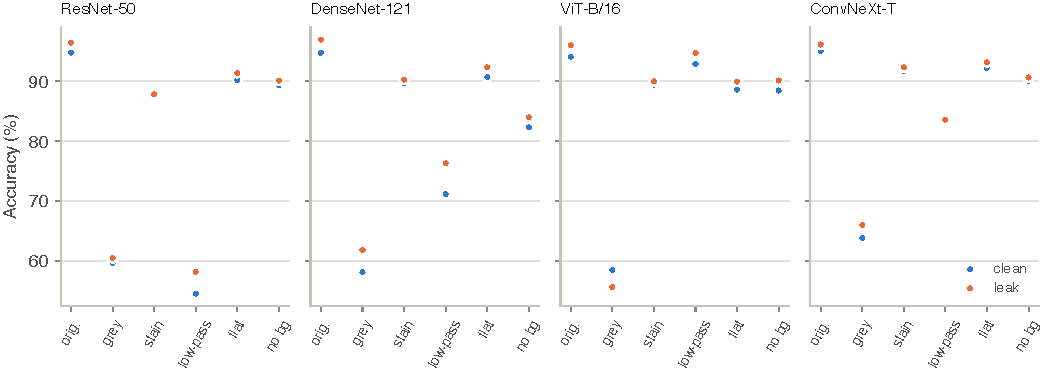
\includegraphics[width=\textwidth]{ablation_arch.pdf}
\caption{Accuracy of leak and clean 2C models under each test-time ablation, per architecture.}
\label{r:fig:ablation-arch}
\end{figure}

{\footnotesize
\setlength{\tabcolsep}{3.5pt}
\begin{longtable}{llrrr}
\caption{Amendment 8 test-time carrier ablations on the Study 2 2C models: leak and clean accuracy (percent, 20 runs each) and the leak advantage (pp).}\label{r:tab:ablation}\\
\toprule
Architecture & Ablation & Leak models & Clean models & Leak $-$ clean \\
\midrule
\endfirsthead
\toprule
Architecture & Ablation & Leak models & Clean models & Leak $-$ clean \\
\midrule
\endhead
\bottomrule
\endfoot
ResNet-50 & original & 96.45\,$\pm$\,0.94 & 94.77\,$\pm$\,1.33 & 1.69 \\
 & grey & 60.41\,$\pm$\,5.61 & 59.56\,$\pm$\,7.27 & 0.84 \\
 & stain\_transfer & 87.81\,$\pm$\,2.85 & 87.76\,$\pm$\,2.77 & 0.05 \\
 & low\_pass & 58.11\,$\pm$\,11.63 & 54.46\,$\pm$\,11.17 & 3.65 \\
 & illumination\_flat & 91.39\,$\pm$\,2.88 & 90.15\,$\pm$\,2.18 & 1.25 \\
 & background\_grey & 90.10\,$\pm$\,2.57 & 89.36\,$\pm$\,1.84 & 0.74 \\
DenseNet-121 & original & 96.94\,$\pm$\,0.78 & 94.73\,$\pm$\,1.50 & 2.21 \\
 & grey & 61.76\,$\pm$\,6.30 & 58.05\,$\pm$\,8.26 & 3.71 \\
 & stain\_transfer & 90.23\,$\pm$\,2.21 & 89.64\,$\pm$\,1.92 & 0.59 \\
 & low\_pass & 76.26\,$\pm$\,6.79 & 71.09\,$\pm$\,5.97 & 5.17 \\
 & illumination\_flat & 92.33\,$\pm$\,2.17 & 90.68\,$\pm$\,3.18 & 1.64 \\
 & background\_grey & 83.98\,$\pm$\,3.72 & 82.27\,$\pm$\,5.20 & 1.71 \\
ViT-B/16 & original & 96.01\,$\pm$\,1.15 & 94.08\,$\pm$\,2.01 & 1.93 \\
 & grey & 55.54\,$\pm$\,5.12 & 58.42\,$\pm$\,7.25 & \textminus{}2.87 \\
 & stain\_transfer & 89.97\,$\pm$\,2.40 & 89.40\,$\pm$\,3.25 & 0.57 \\
 & low\_pass & 94.70\,$\pm$\,1.74 & 92.87\,$\pm$\,2.95 & 1.83 \\
 & illumination\_flat & 89.90\,$\pm$\,2.63 & 88.56\,$\pm$\,3.56 & 1.34 \\
 & background\_grey & 90.12\,$\pm$\,2.73 & 88.44\,$\pm$\,3.54 & 1.68 \\
ConvNeXt-T & original & 96.14\,$\pm$\,1.38 & 95.08\,$\pm$\,1.49 & 1.06 \\
 & grey & 65.94\,$\pm$\,5.38 & 63.77\,$\pm$\,5.85 & 2.16 \\
 & stain\_transfer & 92.31\,$\pm$\,2.68 & 91.69\,$\pm$\,2.52 & 0.61 \\
 & low\_pass & 83.55\,$\pm$\,7.47 & 83.76\,$\pm$\,6.82 & \textminus{}0.20 \\
 & illumination\_flat & 93.20\,$\pm$\,1.62 & 92.21\,$\pm$\,1.87 & 0.98 \\
 & background\_grey & 90.59\,$\pm$\,2.46 & 90.03\,$\pm$\,1.98 & 0.56 \\
\end{longtable}
}


\section{Exploratory: not shared pixels}

In leak cells a third or more of the test crops overlap a training sibling in the source image. Splitting the leak
advantage by overlap (not registered) shows it is as large for crops that share no pixel with any training crop
(\OverlapNo~pp) as for crops that do (\OverlapYes~pp), in the Study~2 models and in all three carrier conditions; stain
transfer removed it in both subsets (\OverlapStainNo\ and \OverlapStainYes~pp). The leak generalises to new cells from a
seen field rather than reflecting memorised pixels.

\begin{figure}[H]
\centering
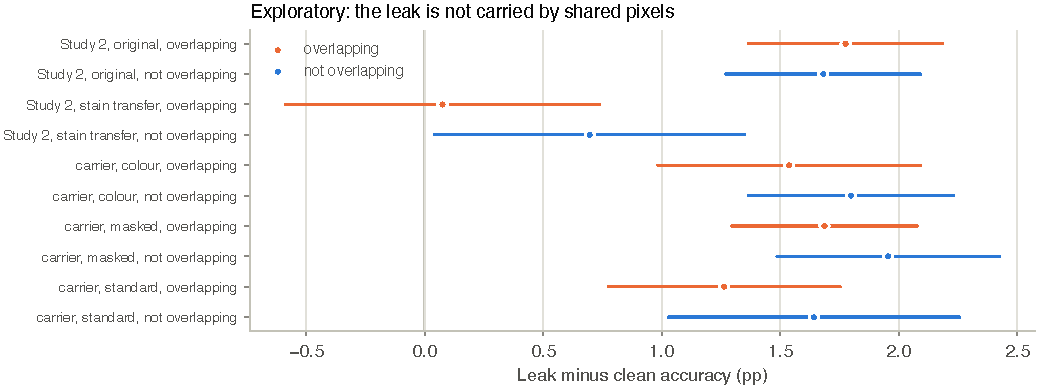
\includegraphics[width=\textwidth]{overlap.pdf}
\caption{Exploratory: the leak advantage on test crops that do or do not share source pixels with a training sibling.}
\label{r:fig:overlap}
\end{figure}

{\footnotesize
\setlength{\tabcolsep}{3.5pt}
\begin{longtable}{llrrrr}
\caption{EXPLORATORY (not registered): leak minus clean accuracy on test crops that do or do not share source pixels with a training sibling (pp; 95\% $t$ interval over architecture--seed--diversity pairs).}\label{r:tab:overlap}\\
\toprule
Condition & Subset & Pairs & Crops & Leak $-$ clean & 95\% CI \\
\midrule
\endfirsthead
\toprule
Condition & Subset & Pairs & Crops & Leak $-$ clean & 95\% CI \\
\midrule
\endhead
\bottomrule
\endfoot
Study 2, original & not overlapping & 80 & 320 & 1.68 & 1.27 to 2.09 \\
Study 2, original & overlapping & 80 & 207 & 1.78 & 1.37 to 2.19 \\
Study 2, stain transfer & not overlapping & 80 & 320 & 0.70 & 0.04 to 1.35 \\
Study 2, stain transfer & overlapping & 80 & 207 & 0.08 & \textminus{}0.59 to 0.74 \\
carrier, colour & not overlapping & 80 & 329 & 1.80 & 1.37 to 2.23 \\
carrier, colour & overlapping & 80 & 206 & 1.54 & 0.98 to 2.09 \\
carrier, masked & not overlapping & 80 & 329 & 1.96 & 1.49 to 2.42 \\
carrier, masked & overlapping & 80 & 206 & 1.69 & 1.30 to 2.08 \\
carrier, standard & not overlapping & 80 & 329 & 1.64 & 1.03 to 2.26 \\
carrier, standard & overlapping & 80 & 206 & 1.26 & 0.77 to 1.75 \\
\end{longtable}
}


\section{No slide-level label prior (F1)}

Over \FoneCells\ discordant CRIC cells from \FoneSlides\ slides, the probability of the slide's majority class was
\FoneEst~pp \emph{lower}, not higher, when the cell's slide was in training (\FoneLo\ to \FoneHi). All six architectures
showed the same sign. Crop-level training raised accuracy as much for discordant cells (\FoneDiscordant~pp) as for
concordant ones (\FoneConcordant~pp; contrast \FoneContrast~pp, \FoneContrastLo\ to \FoneContrastHi): seen slides help each
cell toward its own class, not toward the slide's typical class.

\begin{figure}[H]
\centering
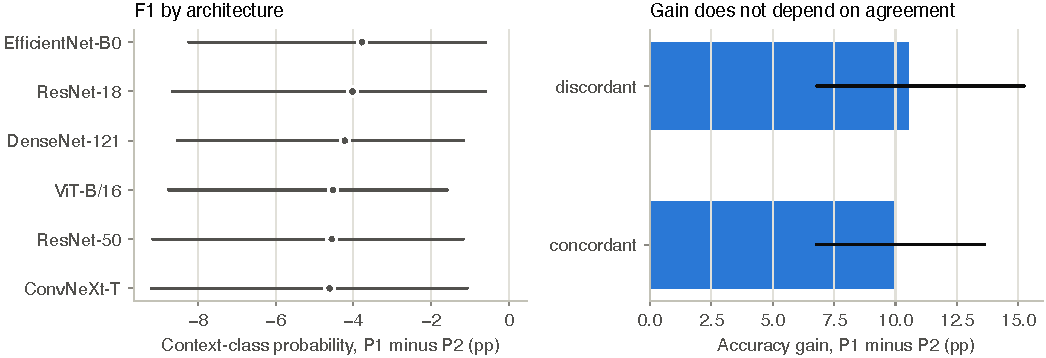
\includegraphics[width=\textwidth]{cric_context.pdf}
\caption{F1 per architecture, and the within-cell accuracy gain for concordant and discordant cells.}
\label{r:fig:cric-context}
\end{figure}

{\footnotesize
\setlength{\tabcolsep}{3.5pt}
\begin{longtable}{lrrrr}
\caption{F1 per architecture (secondary): within-cell P1 $-$ P2 context-class probability on discordant cells (pp) with slide-bootstrap intervals.}\label{r:tab:cricarch}\\
\toprule
Architecture & Estimate & 95\% CI & $p$ & Cells \\
\midrule
\endfirsthead
\toprule
Architecture & Estimate & 95\% CI & $p$ & Cells \\
\midrule
\endhead
\bottomrule
\endfoot
ConvNeXt-T & \textminus{}4.61 & \textminus{}9.19 to \textminus{}1.08 & 0.003 & 1,144 \\
DenseNet-121 & \textminus{}4.22 & \textminus{}8.52 to \textminus{}1.17 & 0.003 & 1,144 \\
EfficientNet-B0 & \textminus{}3.78 & \textminus{}8.22 to \textminus{}0.60 & 0.01 & 1,144 \\
ResNet-18 & \textminus{}4.02 & \textminus{}8.65 to \textminus{}0.61 & 0.01 & 1,144 \\
ResNet-50 & \textminus{}4.56 & \textminus{}9.15 to \textminus{}1.18 & 0.003 & 1,144 \\
ViT-B/16 & \textminus{}4.53 & \textminus{}8.75 to \textminus{}1.60 & $<$0.001 & 1,144 \\
\end{longtable}
}


\section{The gap does not track the fingerprint (F5--F8)}

\begin{figure}[H]
\centering
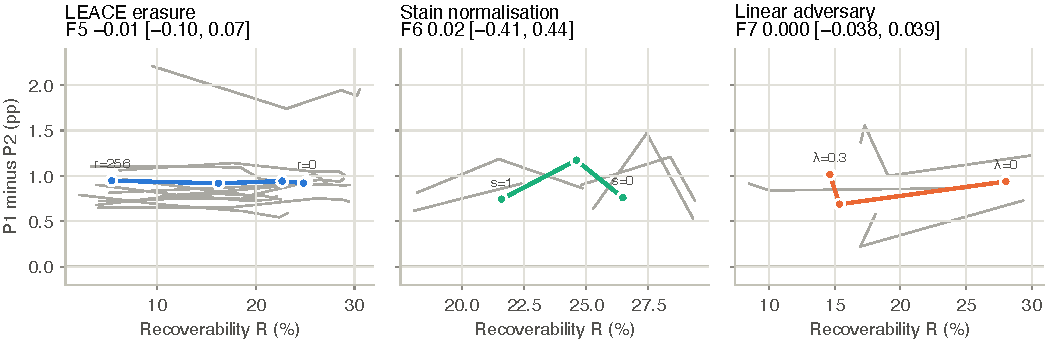
\includegraphics[width=\textwidth]{dose.pdf}
\caption{The P1 $-$ P2 gap against recoverability along three manipulations (grey: architectures; colour: pooled over
architectures that passed the manipulation check, at levels they share; registered in-regime levels only).}
\label{r:fig:dose}
\end{figure}

Rank-256 LEACE erasure cut recoverability from \LeaceRzero\% to \LeaceRtop\% (floor \RFloor\%) in all twelve architectures
while costing P2 \LeaceAccDrop~pp, and the gap stayed at \LeaceGapZero\ to \LeaceGapTop~pp (F5 \FfiveEst, \FfiveLo\ to
\FfiveHi). The probe-matched adversary passed its check in all three architectures, lowering $R$ from
\LinRzeroMin--\LinRzeroMax\% to \LinRstarMin--\LinRstarMax\% inside the regime, with a slope of \FsevenEst\ (\FsevenLo\ to
\FsevenHi). Stain normalisation lowered $R$ only from \NormRzero\% to \NormRtop\% while costing P2 \NormAccDrop~pp, failed
its check for every architecture, and left the gap unchanged (F6 \FsixEst, \FsixLo\ to \FsixHi). Pooled over the
\FeightCells\ included cells, the slope was \FeightEst\ (\FeightLo\ to \FeightHi): even a 20-pp loss of recoverability would
move the gap by at most about 0.1~pp.

\begin{figure}[H]
\centering
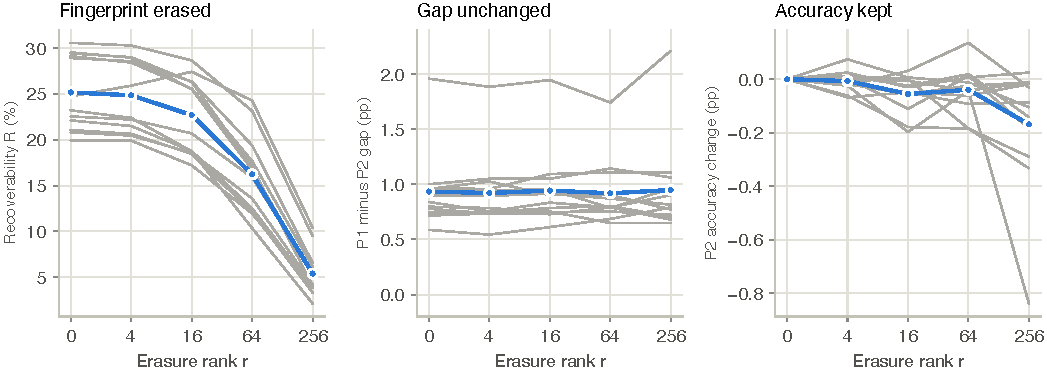
\includegraphics[width=\textwidth]{leace_full.pdf}
\caption{LEACE per architecture (grey) and pooled (blue): recoverability, gap, and P2 accuracy change by erasure rank.}
\label{r:fig:leace-full}
\end{figure}

\begin{figure}[H]
\centering
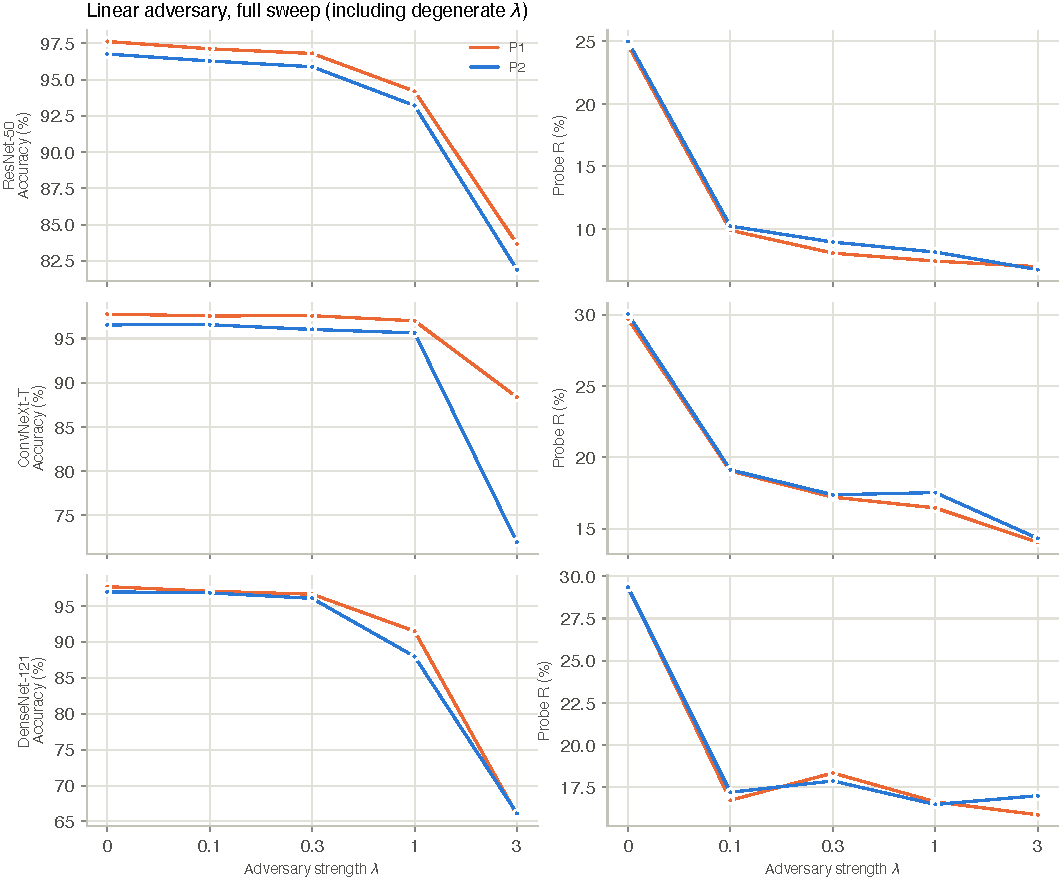
\includegraphics[width=\textwidth]{linadv_full.pdf}
\caption{The full linear-adversary sweep per architecture, including the degenerate strengths ($\lambda=1$ for ResNet-50
and DenseNet-121, $\lambda=3$ for all) where P2 accuracy collapses and which the regime rule excludes.}
\label{r:fig:linadv-full}
\end{figure}

\begin{figure}[H]
\centering
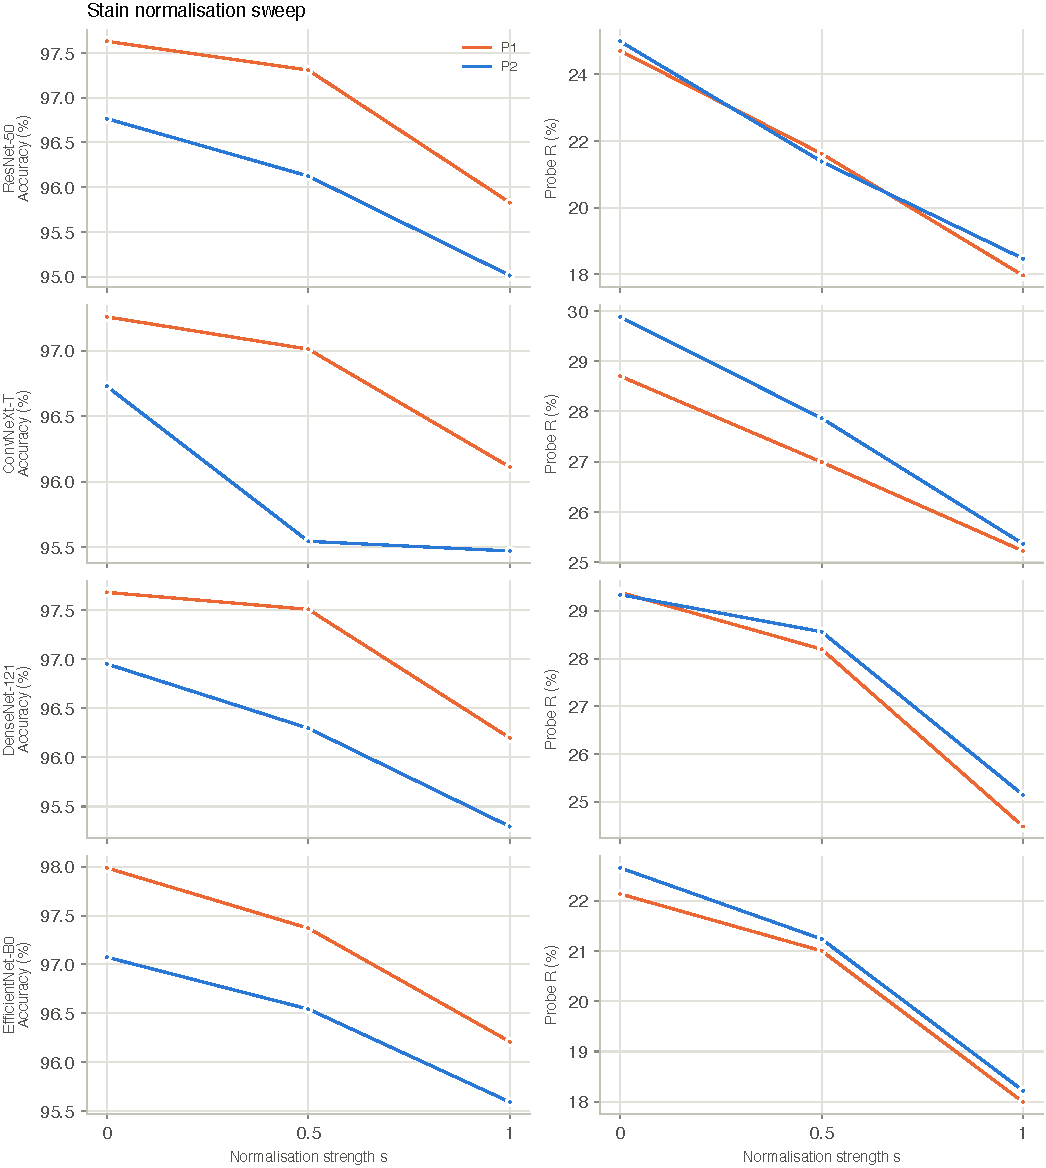
\includegraphics[width=\textwidth]{normalization_full.pdf}
\caption{The stain-normalisation sweep per architecture: accuracy falls for both protocols, recoverability falls only
modestly.}
\label{r:fig:normalization-full}
\end{figure}

{\scriptsize
\setlength{\tabcolsep}{3.5pt}
\begin{longtable}{llp{3.2cm}rrrrl}
\caption{Regimes and manipulation checks of every dose-response arm: levels whose mean P2 accuracy stays within 1 pp of baseline, the strongest such level, recoverability at baseline and there (percent), the class-only floor, and the check (at least a quarter of the above-floor $R$ removed).}\label{r:tab:checks}\\
\toprule
Arm & Architecture & Levels in regime & Strongest & $R_0$ & $R^*$ & Floor & Check \\
\midrule
\endfirsthead
\toprule
Arm & Architecture & Levels in regime & Strongest & $R_0$ & $R^*$ & Floor & Check \\
\midrule
\endhead
\bottomrule
\endfoot
H5 GRL & ResNet-50 & 0, 0.01, 0.03, 0.1, 0.3, 1, 3 & 3 & 24.7 & 17.6 & 1.2 & \pass \\
 & ConvNeXt-T & 0, 0.01, 0.03, 0.1, 0.3, 1, 3 & 3 & 29.5 & 55.1 & 1.2 & \fail \\
F5 LEACE & ResNet-18 & 0, 4, 16, 64, 256 & 256 & 23.2 & 2.1 & 1.2 & \pass \\
 & ResNet-50 & 0, 4, 16, 64, 256 & 256 & 24.7 & 10.4 & 1.2 & \pass \\
 & DenseNet-121 & 0, 4, 16, 64, 256 & 256 & 29.4 & 4.1 & 1.2 & \pass \\
 & EfficientNet-B0 & 0, 4, 16, 64, 256 & 256 & 22.5 & 5.5 & 1.2 & \pass \\
 & MobileNet-V2 & 0, 4, 16, 64, 256 & 256 & 20.8 & 4.2 & 1.2 & \pass \\
 & ViT-B/16 & 0, 4, 16, 64, 256 & 256 & 29.1 & 6.2 & 1.2 & \pass \\
 & ConvNeXt-T & 0, 4, 16, 64, 256 & 256 & 29.5 & 5.2 & 1.2 & \pass \\
 & Swin-T & 0, 4, 16, 64, 256 & 256 & 28.9 & 6.6 & 1.2 & \pass \\
 & RegNetY-1.6GF & 0, 4, 16, 64, 256 & 256 & 21.1 & 3.4 & 1.2 & \pass \\
 & EfficientNetV2-S & 0, 4, 16, 64, 256 & 256 & 19.9 & 3.9 & 1.2 & \pass \\
 & MaxViT-T & 0, 4, 16, 64, 256 & 256 & 22.1 & 3.9 & 1.2 & \pass \\
 & DINOv2 ViT-S/14 & 0, 4, 16, 64, 256 & 256 & 30.5 & 9.5 & 1.2 & \pass \\
F6 normalisation & ResNet-50 & 0, 0.5 & 0.5 & 24.8 & 21.5 & 1.2 & \fail \\
 & DenseNet-121 & 0, 0.5 & 0.5 & 29.4 & 28.4 & 1.2 & \fail \\
 & EfficientNet-B0 & 0, 0.5 & 0.5 & 22.4 & 21.1 & 1.2 & \fail \\
 & ConvNeXt-T & 0 & 0 & 29.3 & 29.3 & 1.2 & \fail \\
F7 linear adv. & ResNet-50 & 0, 0.1, 0.3 & 0.3 & 24.8 & 8.5 & 1.2 & \pass \\
 & DenseNet-121 & 0, 0.1, 0.3 & 0.3 & 29.4 & 18.1 & 1.2 & \pass \\
 & ConvNeXt-T & 0, 0.1, 0.3, 1 & 1 & 29.9 & 17.0 & 1.2 & \pass \\
\end{longtable}
}

{\scriptsize
\setlength{\tabcolsep}{3.5pt}
\begin{longtable}{lrrrrrrr}
\caption{Amendment 8 rank-limited LEACE erasure on every Phase 1 model (20 seeds): accuracy with a refitted head (percent), gap (pp), logistic recoverability $R$, and nearest-centroid recoverability (percent).}\label{r:tab:leace}\\
\toprule
Architecture & Rank & P1 acc. & P2 acc. & Gap & $R$ (P1) & $R$ (P2) & NCC \\
\midrule
\endfirsthead
\toprule
Architecture & Rank & P1 acc. & P2 acc. & Gap & $R$ (P1) & $R$ (P2) & NCC \\
\midrule
\endhead
\bottomrule
\endfoot
ResNet-18 & 0 & 97.90\,$\pm$\,0.37 & 97.31\,$\pm$\,0.61 & 0.59 & 23.1\,$\pm$\,1.2 & 23.2\,$\pm$\,1.1 & 21.0\,$\pm$\,1.0 \\
 & 4 & 97.86\,$\pm$\,0.37 & 97.32\,$\pm$\,0.68 & 0.54 & 22.2\,$\pm$\,1.2 & 22.5\,$\pm$\,1.1 & 19.6\,$\pm$\,1.1 \\
 & 16 & 97.92\,$\pm$\,0.38 & 97.31\,$\pm$\,0.70 & 0.61 & 18.7\,$\pm$\,1.1 & 18.7\,$\pm$\,1.0 & 15.2\,$\pm$\,1.1 \\
 & 64 & 97.81\,$\pm$\,0.37 & 97.12\,$\pm$\,0.81 & 0.69 & 10.5\,$\pm$\,0.8 & 10.2\,$\pm$\,1.0 & 8.1\,$\pm$\,0.8 \\
 & 256 & 97.77\,$\pm$\,0.33 & 96.98\,$\pm$\,1.00 & 0.79 & 2.0\,$\pm$\,0.4 & 2.3\,$\pm$\,0.5 & 1.8\,$\pm$\,0.4 \\
ResNet-50 & 0 & 98.12\,$\pm$\,0.42 & 97.16\,$\pm$\,0.67 & 0.96 & 24.6\,$\pm$\,1.1 & 24.9\,$\pm$\,1.1 & 23.0\,$\pm$\,1.2 \\
 & 4 & 98.12\,$\pm$\,0.45 & 97.09\,$\pm$\,0.72 & 1.02 & 25.9\,$\pm$\,1.5 & 25.9\,$\pm$\,1.2 & 23.5\,$\pm$\,1.2 \\
 & 16 & 98.01\,$\pm$\,0.46 & 97.11\,$\pm$\,0.67 & 0.90 & 27.6\,$\pm$\,1.6 & 27.2\,$\pm$\,1.2 & 24.1\,$\pm$\,1.4 \\
 & 64 & 98.00\,$\pm$\,0.43 & 97.10\,$\pm$\,0.76 & 0.90 & 24.6\,$\pm$\,1.8 & 23.9\,$\pm$\,1.1 & 19.9\,$\pm$\,1.2 \\
 & 256 & 97.91\,$\pm$\,0.43 & 97.14\,$\pm$\,0.72 & 0.77 & 10.7\,$\pm$\,0.9 & 10.1\,$\pm$\,0.8 & 8.7\,$\pm$\,0.8 \\
DenseNet-121 & 0 & 98.24\,$\pm$\,0.32 & 97.52\,$\pm$\,0.67 & 0.72 & 29.5\,$\pm$\,1.3 & 29.2\,$\pm$\,1.3 & 23.7\,$\pm$\,1.3 \\
 & 4 & 98.27\,$\pm$\,0.30 & 97.53\,$\pm$\,0.64 & 0.73 & 29.1\,$\pm$\,1.1 & 28.9\,$\pm$\,1.2 & 22.8\,$\pm$\,1.2 \\
 & 16 & 98.17\,$\pm$\,0.35 & 97.41\,$\pm$\,0.73 & 0.75 & 26.2\,$\pm$\,1.3 & 26.4\,$\pm$\,0.9 & 18.8\,$\pm$\,1.3 \\
 & 64 & 98.19\,$\pm$\,0.25 & 97.54\,$\pm$\,0.78 & 0.65 & 17.1\,$\pm$\,0.8 & 17.0\,$\pm$\,1.2 & 10.8\,$\pm$\,1.1 \\
 & 256 & 97.99\,$\pm$\,0.35 & 97.34\,$\pm$\,0.74 & 0.65 & 3.7\,$\pm$\,0.6 & 4.4\,$\pm$\,0.6 & 2.6\,$\pm$\,0.6 \\
EfficientNet-B0 & 0 & 98.04\,$\pm$\,0.54 & 97.30\,$\pm$\,0.88 & 0.74 & 22.3\,$\pm$\,1.1 & 22.8\,$\pm$\,1.3 & 20.1\,$\pm$\,1.2 \\
 & 4 & 98.05\,$\pm$\,0.53 & 97.30\,$\pm$\,0.87 & 0.75 & 22.0\,$\pm$\,1.0 & 22.4\,$\pm$\,1.4 & 19.5\,$\pm$\,1.2 \\
 & 16 & 98.08\,$\pm$\,0.55 & 97.30\,$\pm$\,0.91 & 0.78 & 20.6\,$\pm$\,1.3 & 20.8\,$\pm$\,1.4 & 17.3\,$\pm$\,1.2 \\
 & 64 & 98.06\,$\pm$\,0.48 & 97.26\,$\pm$\,0.94 & 0.80 & 16.1\,$\pm$\,1.2 & 15.7\,$\pm$\,1.3 & 12.0\,$\pm$\,1.1 \\
 & 256 & 97.99\,$\pm$\,0.49 & 97.29\,$\pm$\,0.75 & 0.70 & 5.5\,$\pm$\,0.8 & 5.5\,$\pm$\,0.9 & 4.2\,$\pm$\,0.6 \\
MobileNet-V2 & 0 & 97.41\,$\pm$\,0.48 & 96.61\,$\pm$\,0.88 & 0.80 & 20.6\,$\pm$\,1.2 & 21.0\,$\pm$\,0.9 & 19.3\,$\pm$\,1.1 \\
 & 4 & 97.41\,$\pm$\,0.52 & 96.62\,$\pm$\,0.91 & 0.78 & 20.2\,$\pm$\,1.0 & 20.7\,$\pm$\,1.1 & 18.3\,$\pm$\,1.0 \\
 & 16 & 97.33\,$\pm$\,0.58 & 96.59\,$\pm$\,0.91 & 0.75 & 18.5\,$\pm$\,1.2 & 18.7\,$\pm$\,1.0 & 15.5\,$\pm$\,1.2 \\
 & 64 & 97.38\,$\pm$\,0.56 & 96.63\,$\pm$\,0.85 & 0.75 & 13.7\,$\pm$\,1.0 & 13.5\,$\pm$\,0.9 & 10.8\,$\pm$\,0.9 \\
 & 256 & 97.19\,$\pm$\,0.49 & 96.47\,$\pm$\,0.80 & 0.72 & 4.2\,$\pm$\,0.8 & 4.2\,$\pm$\,0.6 & 3.5\,$\pm$\,0.6 \\
ViT-B/16 & 0 & 97.83\,$\pm$\,0.75 & 96.83\,$\pm$\,0.80 & 1.00 & 28.8\,$\pm$\,1.2 & 29.4\,$\pm$\,1.2 & 25.1\,$\pm$\,1.3 \\
 & 4 & 97.86\,$\pm$\,0.71 & 96.81\,$\pm$\,0.74 & 1.05 & 28.1\,$\pm$\,1.3 & 28.7\,$\pm$\,1.1 & 23.9\,$\pm$\,1.4 \\
 & 16 & 97.83\,$\pm$\,0.72 & 96.78\,$\pm$\,0.82 & 1.05 & 25.3\,$\pm$\,1.4 & 25.8\,$\pm$\,1.1 & 19.9\,$\pm$\,1.3 \\
 & 64 & 97.88\,$\pm$\,0.68 & 96.73\,$\pm$\,0.76 & 1.14 & 17.6\,$\pm$\,1.3 & 17.7\,$\pm$\,1.4 & 12.7\,$\pm$\,1.2 \\
 & 256 & 97.80\,$\pm$\,0.72 & 96.74\,$\pm$\,0.70 & 1.06 & 6.1\,$\pm$\,0.7 & 6.3\,$\pm$\,1.0 & 4.6\,$\pm$\,0.6 \\
ConvNeXt-T & 0 & 98.20\,$\pm$\,0.36 & 97.30\,$\pm$\,0.72 & 0.90 & 29.3\,$\pm$\,1.3 & 29.7\,$\pm$\,1.5 & 26.3\,$\pm$\,1.6 \\
 & 4 & 98.17\,$\pm$\,0.40 & 97.28\,$\pm$\,0.67 & 0.90 & 28.8\,$\pm$\,1.3 & 29.0\,$\pm$\,1.4 & 25.1\,$\pm$\,1.6 \\
 & 16 & 98.15\,$\pm$\,0.44 & 97.24\,$\pm$\,0.80 & 0.91 & 25.5\,$\pm$\,1.2 & 25.6\,$\pm$\,1.5 & 20.8\,$\pm$\,1.5 \\
 & 64 & 98.14\,$\pm$\,0.37 & 97.27\,$\pm$\,0.73 & 0.87 & 16.8\,$\pm$\,1.1 & 16.6\,$\pm$\,1.1 & 13.0\,$\pm$\,0.9 \\
 & 256 & 98.10\,$\pm$\,0.38 & 97.28\,$\pm$\,0.74 & 0.81 & 5.1\,$\pm$\,0.6 & 5.3\,$\pm$\,0.7 & 4.0\,$\pm$\,0.6 \\
Swin-T & 0 & 98.17\,$\pm$\,0.50 & 97.20\,$\pm$\,0.81 & 0.97 & 29.0\,$\pm$\,1.4 & 28.8\,$\pm$\,1.5 & 25.5\,$\pm$\,1.4 \\
 & 4 & 98.12\,$\pm$\,0.49 & 97.18\,$\pm$\,0.80 & 0.94 & 28.7\,$\pm$\,1.4 & 28.4\,$\pm$\,1.4 & 24.9\,$\pm$\,1.3 \\
 & 16 & 98.19\,$\pm$\,0.48 & 97.23\,$\pm$\,0.77 & 0.96 & 26.5\,$\pm$\,1.1 & 26.2\,$\pm$\,1.5 & 22.0\,$\pm$\,1.4 \\
 & 64 & 98.12\,$\pm$\,0.52 & 97.34\,$\pm$\,0.79 & 0.78 & 19.6\,$\pm$\,1.3 & 19.2\,$\pm$\,1.3 & 15.0\,$\pm$\,1.2 \\
 & 256 & 98.14\,$\pm$\,0.41 & 97.17\,$\pm$\,0.61 & 0.96 & 6.5\,$\pm$\,0.8 & 6.7\,$\pm$\,0.8 & 5.2\,$\pm$\,0.8 \\
RegNetY-1.6GF & 0 & 97.87\,$\pm$\,0.46 & 96.91\,$\pm$\,0.83 & 0.96 & 21.0\,$\pm$\,1.4 & 21.1\,$\pm$\,1.1 & 19.4\,$\pm$\,1.2 \\
 & 4 & 97.80\,$\pm$\,0.42 & 96.85\,$\pm$\,0.83 & 0.96 & 20.5\,$\pm$\,1.3 & 20.8\,$\pm$\,1.4 & 18.9\,$\pm$\,1.1 \\
 & 16 & 97.82\,$\pm$\,0.49 & 96.73\,$\pm$\,0.85 & 1.09 & 18.5\,$\pm$\,1.4 & 18.4\,$\pm$\,1.3 & 15.8\,$\pm$\,1.1 \\
 & 64 & 97.83\,$\pm$\,0.44 & 96.72\,$\pm$\,0.92 & 1.10 & 12.3\,$\pm$\,1.1 & 11.9\,$\pm$\,1.0 & 9.9\,$\pm$\,1.0 \\
 & 256 & 97.72\,$\pm$\,0.42 & 96.62\,$\pm$\,0.85 & 1.10 & 3.3\,$\pm$\,0.7 & 3.4\,$\pm$\,0.6 & 2.7\,$\pm$\,0.7 \\
EfficientNetV2-S & 0 & 97.70\,$\pm$\,0.50 & 96.86\,$\pm$\,1.01 & 0.84 & 19.5\,$\pm$\,1.4 & 20.4\,$\pm$\,1.5 & 17.6\,$\pm$\,1.1 \\
 & 4 & 97.69\,$\pm$\,0.48 & 96.93\,$\pm$\,0.93 & 0.75 & 19.5\,$\pm$\,1.7 & 20.2\,$\pm$\,1.3 & 15.6\,$\pm$\,3.1 \\
 & 16 & 97.70\,$\pm$\,0.51 & 96.86\,$\pm$\,0.89 & 0.83 & 16.7\,$\pm$\,2.1 & 17.8\,$\pm$\,2.0 & 11.5\,$\pm$\,4.2 \\
 & 64 & 97.64\,$\pm$\,0.61 & 96.85\,$\pm$\,0.97 & 0.79 & 11.0\,$\pm$\,3.3 & 12.9\,$\pm$\,2.7 & 7.6\,$\pm$\,3.7 \\
 & 256 & 97.65\,$\pm$\,0.51 & 96.75\,$\pm$\,0.91 & 0.90 & 3.4\,$\pm$\,1.3 & 4.4\,$\pm$\,1.1 & 2.9\,$\pm$\,1.1 \\
MaxViT-T & 0 & 97.88\,$\pm$\,0.46 & 97.10\,$\pm$\,0.83 & 0.78 & 21.6\,$\pm$\,1.2 & 22.6\,$\pm$\,1.5 & 19.1\,$\pm$\,1.3 \\
 & 4 & 97.86\,$\pm$\,0.46 & 97.12\,$\pm$\,0.87 & 0.73 & 20.9\,$\pm$\,1.3 & 22.0\,$\pm$\,1.5 & 18.2\,$\pm$\,1.4 \\
 & 16 & 97.80\,$\pm$\,0.49 & 97.07\,$\pm$\,0.86 & 0.73 & 18.3\,$\pm$\,1.2 & 19.2\,$\pm$\,1.7 & 14.8\,$\pm$\,1.4 \\
 & 64 & 97.90\,$\pm$\,0.49 & 97.10\,$\pm$\,0.86 & 0.79 & 12.4\,$\pm$\,1.0 & 12.6\,$\pm$\,1.7 & 9.4\,$\pm$\,1.0 \\
 & 256 & 97.80\,$\pm$\,0.42 & 97.12\,$\pm$\,0.79 & 0.68 & 3.8\,$\pm$\,0.5 & 4.0\,$\pm$\,0.9 & 3.1\,$\pm$\,0.6 \\
DINOv2 ViT-S/14 & 0 & 95.91\,$\pm$\,0.75 & 93.96\,$\pm$\,1.01 & 1.96 & 30.8\,$\pm$\,0.9 & 30.3\,$\pm$\,1.4 & 26.9\,$\pm$\,1.3 \\
 & 4 & 95.81\,$\pm$\,0.79 & 93.93\,$\pm$\,1.02 & 1.88 & 30.5\,$\pm$\,0.9 & 30.0\,$\pm$\,1.4 & 26.1\,$\pm$\,1.4 \\
 & 16 & 95.70\,$\pm$\,0.76 & 93.76\,$\pm$\,0.97 & 1.94 & 28.4\,$\pm$\,1.1 & 28.9\,$\pm$\,1.3 & 23.8\,$\pm$\,1.4 \\
 & 64 & 95.65\,$\pm$\,0.73 & 93.91\,$\pm$\,1.00 & 1.74 & 23.2\,$\pm$\,1.4 & 23.0\,$\pm$\,1.4 & 16.8\,$\pm$\,1.5 \\
 & 256 & 95.33\,$\pm$\,0.98 & 93.12\,$\pm$\,1.17 & 2.21 & 9.3\,$\pm$\,0.8 & 9.8\,$\pm$\,1.2 & 6.3\,$\pm$\,1.0 \\
\end{longtable}
}

{\footnotesize
\setlength{\tabcolsep}{3.5pt}
\begin{longtable}{lrrrrrr}
\caption{Amendment 8 probe-matched linear adversary (10 seeds): accuracy (percent), gap (pp), and recoverability $R$ (percent; device probe). $\lambda$ above the regime collapses P2 accuracy.}\label{r:tab:linadv}\\
\toprule
Architecture & $\lambda$ & P1 acc. & P2 acc. & Gap & $R$ (P1) & $R$ (P2) \\
\midrule
\endfirsthead
\toprule
Architecture & $\lambda$ & P1 acc. & P2 acc. & Gap & $R$ (P1) & $R$ (P2) \\
\midrule
\endhead
\bottomrule
\endfoot
ResNet-50 & 0 & 97.63\,$\pm$\,0.48 & 96.77\,$\pm$\,0.71 & 0.86 & 24.7\,$\pm$\,1.2 & 25.0\,$\pm$\,0.9 \\
 & 0.1 & 97.12\,$\pm$\,0.29 & 96.28\,$\pm$\,0.44 & 0.84 & 9.9\,$\pm$\,1.1 & 10.2\,$\pm$\,0.9 \\
 & 0.3 & 96.80\,$\pm$\,0.78 & 95.89\,$\pm$\,0.73 & 0.91 & 8.1\,$\pm$\,1.1 & 9.0\,$\pm$\,1.1 \\
 & 1 & 94.20\,$\pm$\,1.88 & 93.21\,$\pm$\,1.61 & 0.99 & 7.4\,$\pm$\,1.3 & 8.1\,$\pm$\,1.4 \\
 & 3 & 83.67\,$\pm$\,8.43 & 81.89\,$\pm$\,8.69 & 1.78 & 7.0\,$\pm$\,1.6 & 6.7\,$\pm$\,1.3 \\
DenseNet-121 & 0 & 97.68\,$\pm$\,0.55 & 96.95\,$\pm$\,0.35 & 0.73 & 29.4\,$\pm$\,1.3 & 29.3\,$\pm$\,1.6 \\
 & 0.1 & 97.04\,$\pm$\,0.60 & 96.81\,$\pm$\,0.77 & 0.22 & 16.7\,$\pm$\,1.4 & 17.2\,$\pm$\,1.5 \\
 & 0.3 & 96.63\,$\pm$\,1.10 & 96.05\,$\pm$\,1.30 & 0.58 & 18.3\,$\pm$\,1.5 & 17.9\,$\pm$\,1.0 \\
 & 1 & 91.48\,$\pm$\,2.44 & 87.96\,$\pm$\,5.59 & 3.52 & 16.6\,$\pm$\,1.0 & 16.5\,$\pm$\,1.8 \\
 & 3 & 65.93\,$\pm$\,7.69 & 66.11\,$\pm$\,9.63 & \textminus{}0.19 & 15.9\,$\pm$\,2.6 & 17.0\,$\pm$\,1.1 \\
ConvNeXt-T & 0 & 97.77\,$\pm$\,0.73 & 96.54\,$\pm$\,0.75 & 1.22 & 29.7\,$\pm$\,1.4 & 30.0\,$\pm$\,1.1 \\
 & 0.1 & 97.56\,$\pm$\,0.75 & 96.56\,$\pm$\,0.78 & 1.00 & 19.0\,$\pm$\,1.4 & 19.1\,$\pm$\,1.6 \\
 & 0.3 & 97.58\,$\pm$\,0.65 & 96.02\,$\pm$\,1.80 & 1.56 & 17.2\,$\pm$\,1.2 & 17.4\,$\pm$\,1.2 \\
 & 1 & 97.00\,$\pm$\,0.69 & 95.63\,$\pm$\,1.18 & 1.37 & 16.5\,$\pm$\,1.9 & 17.5\,$\pm$\,1.5 \\
 & 3 & 88.36\,$\pm$\,3.04 & 71.95\,$\pm$\,28.54 & 16.41 & 14.0\,$\pm$\,1.7 & 14.3\,$\pm$\,3.7 \\
\end{longtable}
}

{\footnotesize
\setlength{\tabcolsep}{3.5pt}
\begin{longtable}{lrrrrrr}
\caption{Amendment 8 Reinhard stain normalisation (10 seeds; strength 0 is the matching Phase 1 run): accuracy (percent), gap (pp), and $R$ (percent).}\label{r:tab:normal}\\
\toprule
Architecture & $s$ & P1 acc. & P2 acc. & Gap & $R$ (P1) & $R$ (P2) \\
\midrule
\endfirsthead
\toprule
Architecture & $s$ & P1 acc. & P2 acc. & Gap & $R$ (P1) & $R$ (P2) \\
\midrule
\endhead
\bottomrule
\endfoot
ResNet-50 & 0 & 97.63\,$\pm$\,0.48 & 96.77\,$\pm$\,0.71 & 0.86 & 24.7\,$\pm$\,1.2 & 25.0\,$\pm$\,0.9 \\
 & 0.5 & 97.31\,$\pm$\,0.58 & 96.12\,$\pm$\,0.68 & 1.19 & 21.6\,$\pm$\,0.7 & 21.4\,$\pm$\,0.9 \\
 & 1 & 95.83\,$\pm$\,0.39 & 95.01\,$\pm$\,1.40 & 0.81 & 18.0\,$\pm$\,1.0 & 18.5\,$\pm$\,1.1 \\
DenseNet-121 & 0 & 97.68\,$\pm$\,0.55 & 96.95\,$\pm$\,0.35 & 0.73 & 29.4\,$\pm$\,1.3 & 29.3\,$\pm$\,1.6 \\
 & 0.5 & 97.51\,$\pm$\,0.47 & 96.30\,$\pm$\,0.61 & 1.21 & 28.2\,$\pm$\,1.1 & 28.6\,$\pm$\,1.4 \\
 & 1 & 96.20\,$\pm$\,0.83 & 95.30\,$\pm$\,0.92 & 0.90 & 24.5\,$\pm$\,1.0 & 25.1\,$\pm$\,0.9 \\
EfficientNet-B0 & 0 & 97.99\,$\pm$\,0.39 & 97.07\,$\pm$\,0.52 & 0.91 & 22.1\,$\pm$\,1.2 & 22.7\,$\pm$\,1.1 \\
 & 0.5 & 97.37\,$\pm$\,0.56 & 96.54\,$\pm$\,0.60 & 0.83 & 21.0\,$\pm$\,1.6 & 21.2\,$\pm$\,1.6 \\
 & 1 & 96.21\,$\pm$\,0.56 & 95.59\,$\pm$\,1.13 & 0.62 & 18.0\,$\pm$\,1.2 & 18.2\,$\pm$\,0.9 \\
ConvNeXt-T & 0 & 97.26\,$\pm$\,0.63 & 96.73\,$\pm$\,0.46 & 0.53 & 28.7\,$\pm$\,1.2 & 29.9\,$\pm$\,1.5 \\
 & 0.5 & 97.01\,$\pm$\,0.76 & 95.54\,$\pm$\,1.44 & 1.47 & 27.0\,$\pm$\,2.0 & 27.9\,$\pm$\,1.0 \\
 & 1 & 96.11\,$\pm$\,1.24 & 95.47\,$\pm$\,1.06 & 0.64 & 25.2\,$\pm$\,1.9 & 25.4\,$\pm$\,1.1 \\
\end{longtable}
}


\section{Grad-CAM sees no difference}

Leak and clean models placed the same share of Grad-CAM attribution outside the cell mask (\CamBgAttribution\% on average,
against a background pixel share of \CamBgPixels\%; leak minus clean \CamLeakEst~pp, \CamLeakLo\ to \CamLeakHi). The maps
depended on the trained head (median Spearman \CamSpearman\ with a random-head map), so the absence of a difference is not a
failure of the method's sanity check.

\begin{figure}[H]
\centering
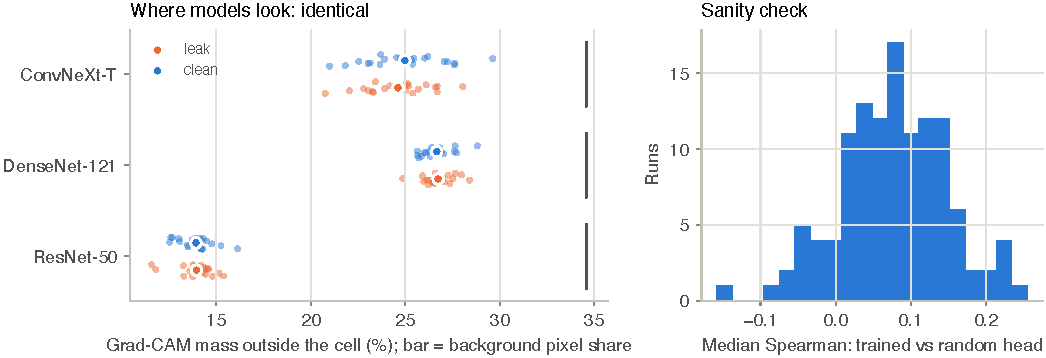
\includegraphics[width=\textwidth]{gradcam.pdf}
\caption{Left: per-run Grad-CAM attribution outside the cell for leak and clean models (bar: background pixel share).
Right: agreement of each run's maps with random-head maps.}
\label{r:fig:gradcam}
\end{figure}

{\footnotesize
\setlength{\tabcolsep}{3.5pt}
\begin{longtable}{llrrr}
\caption{Grad-CAM (descriptive): share of positive attribution outside the cell mask and background pixel share (percent, 20 runs each), and the median Spearman correlation with a random-head map.}\label{r:tab:gradcam}\\
\toprule
Architecture & Models & Attribution outside & Background pixels & Random-head $\rho$ \\
\midrule
\endfirsthead
\toprule
Architecture & Models & Attribution outside & Background pixels & Random-head $\rho$ \\
\midrule
\endhead
\bottomrule
\endfoot
ResNet-50 & leak & 13.9\,$\pm$\,1.0 & 34.6\,$\pm$\,0.5 & 0.085 \\
 & clean & 13.9\,$\pm$\,0.9 & 34.6\,$\pm$\,0.5 & 0.115 \\
DenseNet-121 & leak & 26.7\,$\pm$\,0.8 & 34.6\,$\pm$\,0.5 & 0.044 \\
 & clean & 26.7\,$\pm$\,0.8 & 34.6\,$\pm$\,0.5 & 0.057 \\
ConvNeXt-T & leak & 24.6\,$\pm$\,1.8 & 34.6\,$\pm$\,0.5 & 0.077 \\
 & clean & 25.0\,$\pm$\,2.2 & 34.6\,$\pm$\,0.5 & 0.076 \\
\end{longtable}
}


\chapter{The mechanism by elimination}
\label{r:ch:elimination}

\begin{figure}[H]
\centering
\begin{adjustbox}{max width=\textwidth}
\begin{tikzpicture}[node distance=2.5mm and 6mm]
\node[box=38mm] (q) {Where does the leaked advantage live?};
\node[bad=40mm, below left=6mm and -8mm of q] (bg) {Background context\\\footnotesize H4 null; F3 survives masking; test-time removal keeps \RecBgKeep\%};
\node[bad=40mm, below=of bg] (pix) {Literally shared pixels\\\footnotesize exploratory: equal for non-overlapping crops};
\node[bad=40mm, below=of pix] (prior) {Slide-level label prior\\\footnotesize F1 reversed; equal gain when discordant};
\node[bad=40mm, below=of prior] (code) {Linear field-identity code\\\footnotesize F5, F7, F8: $R$ cut up to \RecoveryCutMax\%, gap flat};
\node[bad=40mm, below=of code] (sal) {Visible to saliency\\\footnotesize Grad-CAM identical for leak and clean};
\node[done=40mm, below right=6mm and -8mm of q] (colour) {Tied to the field's colour rendering\\\footnotesize F2: stain transfer removes \RecStainRemove\%};
\node[gold=40mm, below=of colour] (aug) {Not prevented by colour jitter\\\footnotesize F4 null};
\node[box=40mm, below=8mm of aug] (account) {Account: class evidence calibrated to each seen field's appearance};
\draw[flow] (q) -- (bg); \draw[flow] (q) -- (colour);
\draw[flow] (colour) -- (aug); \draw[flow] (aug) -- (account);
\end{tikzpicture}
\end{adjustbox}
\caption{The mechanism by elimination. Red: candidate carriers ruled out; green: the one intervention that removed most
of the advantage; gold: the qualification that keeps the account modest.}
\label{r:fig:elimination}
\end{figure}


Taken together with Study~2's H4 and H5, the follow-up narrows how models use the leak. The advantage does not need a
background (F3, test-time removal, H4). It is not memorisation of shared pixels (exploratory). It is not a slide-level label
prior (F1, reversed). It is not carried by a separable, linearly decodable field code: erasing that code in closed form, or
suppressing it with an adversary that cannot hide it from a linear probe, cut recoverability by \RecoveryCutMin--\RecoveryCutMax\%
without moving the gap (F5, F7, F8). What remains is that the advantage depends on the cell being rendered as its own field
renders cells: matching a test cell's colour statistics to another field of the same class removed most of it (F2).

The simplest account consistent with all of this is that a model trained on a field's siblings calibrates its class
evidence to that field's appearance (stain, colour balance, and the texture they produce in the cell itself), so cells
from a seen field sit further inside their class region. Random colour jitter during training did not prevent this (F4),
presumably because jitter perturbs each image around its own appearance and leaves the field-specific structure of that
appearance learnable. This account is a reading of the evidence, not a registered result, and the F2--F4 tension is the
part of it most in need of a direct test (for example, stain transfer applied to colour-augmented models).

\begin{decisionbox}{Decodable is not used, and saliency is not use}
Study~1 established \emph{availability}: a probe recognised fields at 109 times chance. The follow-up shows that availability
and use come apart: the identity a probe reads can be removed almost entirely without touching the inflation, in line with
evidence from language models that probe-decodable information need not be what a model relies
on~\citep{elazar2021amnesic,ravichander2021probing}. Grad-CAM showed leak and clean models attending to the same places; a
saliency audit would have cleared both.
\end{decisionbox}
